\newpage
\section{Функциональные требования}
\begin{figure}[h]
\center{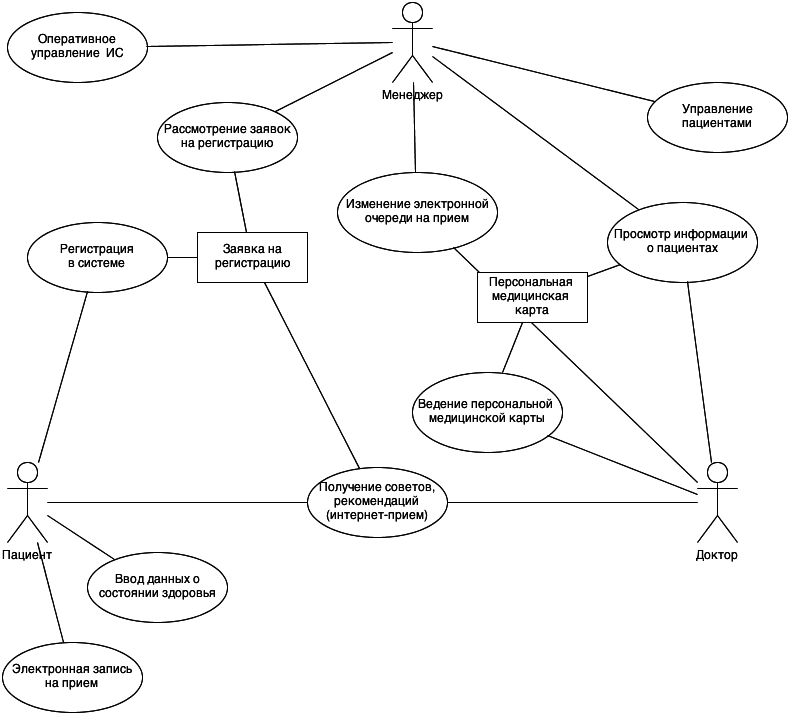
\includegraphics[width=0.9\linewidth]{main_use_case.eps}}
\caption{Варианты использования системы}
\label{ris:main_use_case}
\end{figure}

На рисунке \ref{ris:main_use_case} приведена диаграмма вариантов использования
системы. Рассмотрим каждую роль подробнее.

\subsection{Пациент}
Данная роль является основной в разрабатываемой системе. Пользователи с данной
ролью будут иметь доступ к своим медицинским данным, возможность просмотра и
изменения (в рамках установленных границ) своего расписания, возможность
общаться с лечащим доктором, просмотр медицинских заключений, выданных доктором.
Также пользователи могут иметь возможность просмотра новостных рассылок сайта.

Основные варианты использования системы:

\begin{enumerate}
  \item расписание:
  \begin{enumerate}
    \item время приема лекарств;
    \item даты обследований;
    \item даты приемов у врача;     
  \end{enumerate}
  \item регистрация в системе - процесс регистрации в ситеме состоит из
  следующих этапов:
  \begin{enumerate}
    \item заполнение и подача электронной заявки на регистрацию. Подать заявку
    (на даном этапе анализа моделирования) могут только пациенты, проходящие
    лечение в Кузбасском кардиоцентре. 
    В заявке необходимо указать ФИО пациента и его матери (отца или опекуна), номер сотового телефона (для отправки на него аутентификационных данных), номер медицинской карточки, придуманный пользователем пароль;
    \item получение отказа или подтверждение на регистрацию в системе. В случае
    успешной регистрации пользователь получит аутентификационные данные для
    входа в систему. В атуентификационные данные входить сгенерированный логин и
    оставленный пользователем пароль.
  \end{enumerate}
  \item ввод показателей о состоянии здоровья согласно расписанию составленному
лучащим врачом пациента. Список показателей для мониторинга также составляется
врачом индивидуально для каждого пациента;
  \item электронная запись - процесс записи пациента к врачу, на обследование,
процедуры и другие услуги предоставляемы лечащим заведением с целью получать
актуальные данные о состоянии здоровья пациента и оперативно вносить изменения в процесс лечения или мониторинга;
\end{enumerate}

\subsection{Доктор}
Не менее важной ролью в системе является роль доктора. Пользователи с данной ролью могут иметь доступ к медицинским данным тех пациентов, которые к ним приписаны, просматривать их расписания, возможность связаться с пациентом для оказания консультации по тому или иному вопросу. Специфичными конкректно для роли доктора являются доступ к расписанию приема доктора, медицинским заключениям, выпискам лекарств.

Основные варианты использования:	
\begin{enumerate}
  \item ведение персональной медицинской карты:
  \begin{enumerate}
  	\item заполнение данных о приеме;
  	\item заполнение рекомендательных данных по улучшениею состояния пациента
  	или поддержания состояния в устойчивом положении;
  	\item агрегирование и анализ результатов исследований, обследований.
  \end{enumerate}
  \item просмотр информации о пациентах - возможность врача получить доступ к
  любой необходимой, имеющейся в базе, инфрмации о ведомом пациенте (или другом
  пациенте с его согласия) для анализа состояния пациента;
  \item назначение обследований;
  \item назначение лекарственных препаратов. 
\end{enumerate}

\subsection{Менеджер}
Данная роль является связущей (в плане управления) всех участников системы. У
пользователей с данной ролью есть доступ к персональным немедицинским данным
пациентов и докторов, заявкам на регистрацию, электронной очереди, некоторой
общестатистической информации.

Основные варианты использования:

\begin{enumerate}
  \item оперативное управление системой - мониториг состояния системы и
  консульация пользователей по работе с ней;
  \item рассмотрение заявок на регистрацию - обработка всех поступающих заявок и
  принятие решения о подтверждении или отклонении заявки;
  \item изменение электронной очереди на прием;
  \item оценка эффективности лечения;
  \item оценка качества лечения.
\end{enumerate}

\subsection{Электронный (интернет) прием}
Является общим (кооперирующим) функционалом для пациентов и докторов. Необходим
в случае невозможности пациента явится на личный прием к врачу, а также если сам
врач не может лично посетить пациента, например в случае отъезда того или иного
участника приема. Должна быть возможность провести удаленный прием с фиксацией
всех данных полученных в результате приема. Различие в использовании данной
функциональной возможности состоит в том, что пациент передает врачу и системе
свои медицинские данные и получает медицинское заключение, а врач наоборот, на
основании данных пациента выписывает лекарства и выдает заключение.

\subsection{Интернет-консультация}
Интернет-консультация должна сократить нагрузку на лечащего врача, за счет
делегирования части обязанностей на консультантов. В случае если консультант не
может помочь пациенту, пациента можно отправить на интернет-прием или на личный
прием к врачу.
